%% LyX 2.3.6.1 created this file.  For more info, see http://www.lyx.org/.
%% Do not edit unless you really know what you are doing.
\documentclass[english]{article}
\usepackage[T1]{fontenc}
\usepackage[latin9]{inputenc}
\usepackage{geometry}
\geometry{verbose,tmargin=2.5cm,bmargin=2.5cm,lmargin=2.5cm,rmargin=2.5cm}
\usepackage{graphicx}

\makeatletter

%%%%%%%%%%%%%%%%%%%%%%%%%%%%%% LyX specific LaTeX commands.
%% Because html converters don't know tabularnewline
\providecommand{\tabularnewline}{\\}

\makeatother

\usepackage{babel}
\begin{document}
{[}SPLIT\_HERE{]}
\begin{enumerate}
\item \textbf{{[}DHS/PRELIM/9597/2016/P1/Q1{]} }

In Olympic diving, scoring is done by a panel comprising a minimum
of 3 judges. The highest and lowest scores are dropped to eliminate
the extremes. The raw score is computed by summing the middle scores.
The raw score is then multiplied by the level of difficulty to give
the total score. 

Sample scoring for a 5-judges panel: Scores: 

6.5, 6, 6.5, 6, 5.5 

Lowest (5.5) and highest (6.5) scores dropped 

Raw Score = 18.5 (6.5 + 6 + 6) 

Total Score = Score (18.5) x Difficulty Level (1.5) = 27.75 

\texttt{DIVE1.TXT} contains the countries, difficulty levels and 5-judges
scores for a diving competition. 

\subsection*{Task 1.1 }

Write program code to determine the podium winners of the competition.
Your program should output the medal (Gold, Silver, Bronze), country
name and the total score (to 2 decimal places). 

Sample output:

\noindent %
\noindent\begin{minipage}[t]{1\columnwidth}%
\texttt{Gold: China 45.90 }

\texttt{Silver: Malaysia 39.20}

\texttt{Bronze: United States 36.00 }%
\end{minipage}

\subsection*{Evidence 1: }

Program code. \hfill{}{[}5{]}

\subsection*{Evidence 2: }

Screenshot of output. \hfill{}{[}1{]}

In most international competitions with more than five judges, the
3/5 method is used. The middle 5 numbers are added and then multiplied
by the difficulty of the dive and then multiplied again by 0.6. \texttt{DIVE2.TXT}
contains the countries, difficulty levels and 9-judges scores for
a diving competition. 

\subsection*{Task 1.2 }

Write program code to determine the podium winners of the competition.
Your program should output the medal (Gold, Silver, Bronze), country
name as well as the total score (to 2 decimal places). 

\subsection*{Evidence 3: }

Program code. \hfill{}{[}8{]}

\subsection*{Evidence 4: }

Screenshot of output. \hfill{}{[}1{]}

{[}SPLIT\_HERE{]}
\item \textbf{{[}DHS/PRELIM/9597/2016/P1/Q2{]} }

Quicksort is an efficient sorting algorithm to order values in an
array. 

\subsection*{Task 2.1 }

Write a recursive quicksort method to sort the values in the text
file \texttt{DATA.TXT} in descending order. 

\subsection*{Evidence 5: }

Program code for Task 2.1. \hfill{}{[}4{]}

\subsection*{Evidence 6:}

Screenshot of output. \hfill{}{[}2{]}

\subsection*{Task 2.2 }

Using a suitable data structure, convert the recursive quicksort in
Task 2.1 to one using iteration. Confirm the correctness of your iterative
quicksort on the data set used in Task 2.1 

\subsection*{Evidence 7:}

Program code for Task 2.2.\hfill{}{[}8{]}

\subsection*{Evidence 8: }

Screenshot of output. \hfill{}{[}1{]}

{[}SPLIT\_HERE{]}
\item \textbf{{[}DHS/PRELIM/9597/2016/P1/Q3{]} }

A Pokemon Go fan who nicknames himself Pokeboy wishes to manage his
Pokemon collection using a binary search tree. Each binary search
tree node stores the name together with the numbers of that particular
Pokemon and candies collected, as well as a reference to a linked
list. Each linked list node stores the combat power (CP) of a Pokemon.
The binary search tree is organised in ascending Pokemon name order.
Each linked list is organised in descending order of CP. For ease
of reference, we shall name this composite data structure Poketree. 

\subsection*{Task 3.1 }

Using object-oriented programming, construct appropriate classes to
initialise, insert and display the contents of the Poketree. In your
main driver program, write code to initialise a Poketree with the
first Pokemon collected which is randomly generated from the contents
in the file \texttt{POKEMONS.TXT} as well as a randomly generated
CP in the range 10 to 200 inclusive. When a Pokemon is caught, 3 candies
of that kind are also added to the candies count of the Poketree binary
search tree node.

\subsection*{Evidence 9: }

Program code for class definition, initialisation and display methods.\hfill{}
{[}7{]}

\subsection*{Evidence 10:}

Screenshot output to show contents of Poketree with first Pokemon
inserted.\hfill{} {[}1{]}

\subsection*{Task 3.2 }

Write a class method \texttt{insert()} and the necessary main driver
program code to insert another 23 randomly generated Pokemons and
their corresponding CPs into the Poketree. 

\subsection*{Evidence 11: }

Program code for Task 3.2.\hfill{} {[}4{]}

\subsection*{Evidence 12:}

Screenshot to show updated contents of Poketree.\hfill{} {[}1{]}

Apart from collecting Pokemons, one can also evolve Pokemons. When
a new Pokemon is evolved, its previous incarnation is deleted from
the Poketree and its new incarnation either inserted (if its kind
is not previously collected) or updated (if its kind is previously
collected) to the Poketree. Evolving also requires a set amount and
type of Pokemon candy. If there is insufficient Pokemon candies, Pokeboy's
preferred action is to exchange (i.e. delete) existing Pokemons of
the same species for candies, starting from the Pokemon with the lowest
CP. Each Pokemon can be exchanged for one candy. Pokeboy also wishes
to keep at least 2 Pokemons of the same species in his collection
(well he is a Pokemon fan). The text file \texttt{CANDIES.TXT} contains
the candies requirement for evolvement. 

\subsection*{Task 3.3 }

Write a Boolean class method \texttt{can\_evolve(pokemon)} to determine
if a particular Pokemon can evolve by Pokeboy's preference. A Pokemon
can evolve if there are sufficient candies or it is possible to exchange
candies, leaving a minimum of 2 Pokemons of that species.

Write a class method evolve(pokemon) which will evolve a Pokemon using
\texttt{can\_evolve(pokemon)}. 

Add necessary class method(s) and main driver program code to evolve
all evolvable Pokemons. 

\subsection*{Evidence 13: }

Program code for Task 3.3.\hfill{} {[}7{]}

\subsection*{Evidence 14:}

Screenshot(s) to show evolution.\hfill{} {[}1{]}

\subsection*{Task 3.4 }

Write a class method \texttt{most\_poke()} to output the frequency
and most collected Pokemon(s) collected by Pokeboy. 

Add necessary program code to exercise \texttt{most\_poke()}.

\subsection*{Evidence 15: }

Program code for Task 3.4.\hfill{} {[}4{]}

\subsection*{Evidence 16:}

Screenshot for Task 3.4. \hfill{}{[}1{]}

\subsection*{Task 3.5}

Pokeboy aspires to join the Catch Them All club. The Catch Them All
club is a group of elites who have managed to catch every species
of Pokemon at least once. Write a class method \texttt{catch\_them\_all()}
to either output the message \textquotedbl Welcome to the club! You
have caught them all!\textquotedbl{} or output the number and remaining
Pokemon names yet to be caught.

Add necessary program code to exercise \texttt{catch\_them\_all()}. 

\subsection*{Evidence 17:}

Program code for Task 3.5.\hfill{} {[}6{]}

\subsection*{Evidence 18: }

Screenshot for annotated test cases. \hfill{}{[}2{]}

\subsection*{Task 3.6 }

After some time, it becomes necessary to reorganise the binary search
tree to ensure optimal search performance. Write program code to rebalance
the binary search tree and include as comments your strategy to do
this. You should output the roots and heights of the old and new binary
search trees.

\subsection*{Evidence 19:}

Program code for Task 3.6.\hfill{} {[}5{]}

\subsection*{Evidence 20:}

Screenshot.\hfill{} {[}1{]}

{[}SPLIT\_HERE{]}
\item \textbf{{[}DHS/PRELIM/9597/2016/P1/Q4{]} }

A magic index in an array A is defined to be an index such that \texttt{A{[}i{]}
= i}. 

\subsection*{Task 4.1 }

Given a sorted array of distinct integers, write a brute force iterative
method \texttt{magic\_index(A)} to find a magic index if one exists.
If a magic index does not exist, return -1. 

\subsection*{Evidence 21: }

Function code for \texttt{magic\_index(A)} and relevant driver code.\hfill{}
{[}5{]}

\subsection*{Evidence 22: }

Screenshot of output.\hfill{} {[}2{]}

\subsection*{Task 4.2 }

Write an efficient recursive method \texttt{magic\_index\_duplicates(A)}
to find a magic index for an array containing non-distinct values.
If a magic index does not exist, return -1.

\subsection*{Evidence 23: }

Function code for \texttt{magic\_index\_duplicates(A)} and relevant
driver code. \hfill{} {[}6{]}

\subsection*{Evidence 24:}

Screenshot of output. \hfill{} {[}2{]}

A child is running up a staircase with n steps and can hop either
1, 2 or 3 steps at a time. 

\subsection*{Task 4.3 }

Write a brute force recursive method to count how many possible ways
the child can run up the stairs. 

\subsection*{Evidence 25: }

Function code and relevant driver code.\hfill{} {[}5{]}

\subsection*{Evidence 26: }

Screenshot of output.\hfill{} {[}2{]}

\subsection*{Task 4.4 }

Optimise your brute force recursive solution in Task 4.3 by eliminating
unnecessary recomputations.

\subsection*{Evidence 27: }

Function code and relevant driver code.\hfill{} {[}6{]}

\subsection*{Evidence 28:}

Screenshots showing annotated test cases. \hfill{} {[}2{]}

{[}SPLIT\_HERE{]}
\item \textbf{{[}DHS/PRELIM/9597/2016/P2/Q1{]} }

GovBuy is a Government Digital Services initiative that helps government
employees buy microservices (small pieces of software that can be
deployed independently), software libraries, non-critical bug fixes
or even customised hardware from independent contractors. 

The platform allows government employees to post a task. Anyone can
bid to take on the task during the bidding period. The reverse auction
starts at \$5,000 and the lowest bid wins.

The winner works on the task and submits completed code to the team.
If the code meets the acceptance criteria before the deadline, the
winner is sent a cheque for the work.

The current prototype platform is a web interface:
\begin{center}
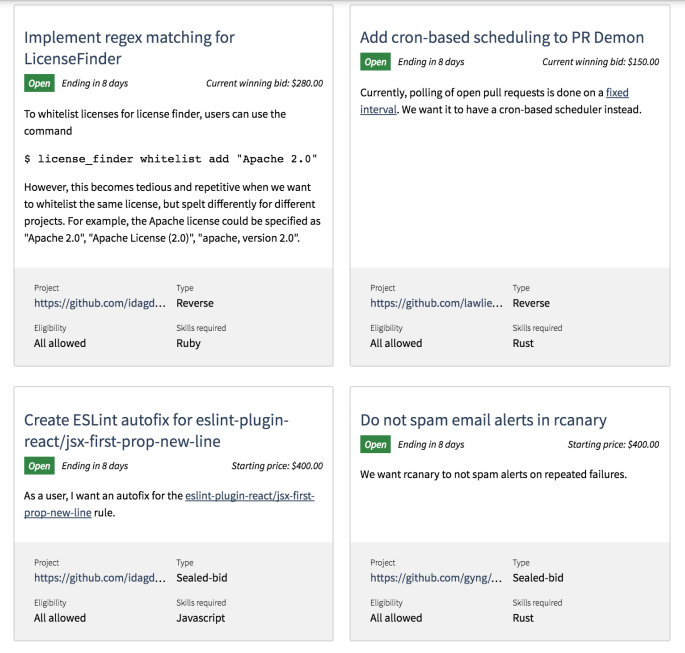
\includegraphics[width=0.5\paperwidth]{C:/Users/Admin/Desktop/Github/question_bank/LyX/static/img/9597-DHS-2016-P2-Q1-1}
\par\end{center}
\begin{enumerate}
\item The agency in charge wishes to develop mobile native versions of the
platform for Android and iOS. The following diagram shows the expected
workflow. 
\begin{center}
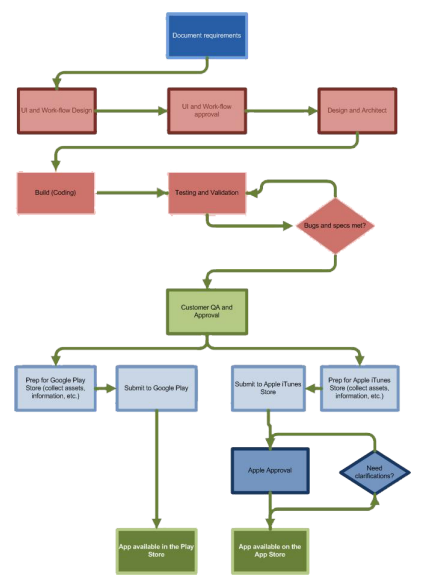
\includegraphics[width=0.5\paperwidth]{C:/Users/Admin/Desktop/Github/question_bank/LyX/static/img/9597-DHS-2016-P2-Q1-2}
\par\end{center}
\begin{enumerate}
\item Create a PERT chart from the above workflow diagram. You may assume
the following durations from the activity table below.\hfill{} {[}4{]}
\noindent \begin{center}
\begin{tabular}{|c|l|c|}
\hline 
Phase & Description & Duration (weeks)\tabularnewline
\hline 
A & Gather and document requirements & 2\tabularnewline
\hline 
B & UI and workflow design and approval & 3\tabularnewline
\hline 
C & Design and architect & 4\tabularnewline
\hline 
D & Build (coding) & 7\tabularnewline
\hline 
E & Testing and validation & 3\tabularnewline
\hline 
F & Customer QA and approval & 2\tabularnewline
\hline 
G & Prepare and submit to Google Play Store & 1\tabularnewline
\hline 
H & Prepare and submit to Apple App Store & 1\tabularnewline
\hline 
I & Apple approval & 1\tabularnewline
\hline 
\end{tabular} 
\par\end{center}
\item From the PERT chart, state the critical path and the minimum project
completion time. \hfill{}{[}2{]}
\item Describe two benefits which can be gained by producing a PERT chart.\hfill{}
{[}2{]}
\item Describe and give an example of a dependent activity. \hfill{}{[}2{]}
\item Describe and give an example of a concurrent activity.\hfill{} {[}2{]}
\end{enumerate}
\item The project manager decides he needs another diagrammatic tool to
monitor the project progress.
\begin{enumerate}
\item Create a Gantt chart for the project.\hfill{} {[}3{]}
\item Explain how the Gantt chart can help the developers in carrying out
their work.\hfill{} {[}2{]}
\end{enumerate}
\item Describe two activities to mark the closure of the project. \hfill{}{[}4{]}
\item Cybersecurity is of paramount concern when it comes to government
web services. Using suitable examples, explain the following cybersecurity
exploits and suggest how they can be mitigated. 
\begin{enumerate}
\item Cross site scripting \hfill{}{[}3{]}
\item Code injection \hfill{}{[}3{]}
\item Denial of service attack \hfill{}{[}3{]}
\end{enumerate}
\item The platform will be hosted using cloud computing. 
\begin{enumerate}
\item Explain why the cloud is a suitable hosting platform. \hfill{}{[}2{]}
\item Use suitable example to illustrate the concepts of IaaS, PaaS and
SaaS. \hfill{}{[}6{]}
\end{enumerate}
\item What ethical considerations should bidders bear in mind when bidding
for tasks on an open source platform such as GitHub?\hfill{} {[}2{]}
\end{enumerate}
{[}SPLIT\_HERE{]}
\item \textbf{{[}DHS/PRELIM/9597/2016/P2/Q2{]} }

The current GovBuy prototype supports two types of reverse auctions:
a standard reverse auction and a sealed bid auction. 

A standard reverse auction is one where bids begin at \$5,000. The
lowest possible bid is \$1, and an auction automatically ends once
a \$1 bid has been submitted. Bidders are allowed to submit multiple
bids throughout the duration of the auction. Bidders will see whether
they are the winning bidder after submitting a bid, and will have
an opportunity to submit a lower bid if the auction is still running.
The GitHub user names of participating bidders are hidden during the
auction. At the end of the auction, all bidders' GitHub accounts and
bid amounts will be unsealed and posted on the GovBuy platform. A
sealed bid auction is a type of reverse auction. Each bidder is allowed
to submit only one bid in an auction. Once a bid is submitted, the
bidder may not submit a second bid for the same auction. The lowest
bidder at the conclusion of the auction will still win the auction.
In the event that one or more bidders have the same bid amount, the
bidder who was first to submit the lowest bid amount will win the
auction. All bids will stay sealed until the end of the auction. A
bidder will not know the amounts other bidders have bidded on the
auction, or how many bids have been submitted. At the end of the auction,
all bidders' GitHub accounts and bid amounts will be unsealed and
posted on the GovBuy platform. 
\begin{enumerate}
\item Illustrate the types of reverse auctions in a class UML diagram. \hfill{}{[}5{]}
\item Using your illustration, explain the following OOP concepts: 
\begin{enumerate}
\item encapsulation \hfill{}{[}2{]}
\item inheritance \hfill{}{[}2{]}
\item polymorphism \hfill{} {[}2{]}
\end{enumerate}
\end{enumerate}
{[}SPLIT\_HERE{]}
\item \textbf{{[}DHS/PRELIM/9597/2016/P2/Q3{]}}

The following code shows the program \texttt{mystery1}. 

\noindent %
\noindent\begin{minipage}[t]{1\columnwidth}%
\texttt{epsilon = 0.01 }

\texttt{step = epsilon {*}{*} 2}

\texttt{num\_guesses = 0}

\texttt{ans = 0.0 }

\texttt{while abs(ans {*}{*} 2 - x) >= epsilon and ans {*} ans <=
x: }

\texttt{\qquad{}ans += step }

\texttt{\qquad{}num\_guesses += 1 }

\texttt{print(\textquotedbl\#Guesses =\textquotedbl , num\_guesses) }

\texttt{print(\textquotedbl Answer =\textquotedbl , ans) }%
\end{minipage}
\begin{enumerate}
\item Running the program with \texttt{x = 25} gives the following output: 

\noindent\begin{minipage}[t]{1\columnwidth}%
\texttt{\#Guesses = 49990 }

\texttt{Answer = 4.999000000001688}%
\end{minipage}
\begin{enumerate}
\item What do you think is the purpose of the program \texttt{mystery1}?
\hfill{} {[}2{]}
\item Comment on the efficiency of program mystery1. \hfill{}{[}2{]}
\end{enumerate}
\item An alternative version, program \texttt{mystery2} is provided as follows. 

\noindent\begin{minipage}[t]{1\columnwidth}%
\texttt{epsilon = 0.01}

\texttt{num\_guesses = 0}

\texttt{low = 0}

\texttt{high = x}

\texttt{ans = (high + low) / 2 }

\texttt{while abs(ans {*}{*} 2 - x) >= epsilon:}

\texttt{\qquad{}num\_guesses += 1 }

\texttt{\qquad{}if ans {*}{*} 2 < x: }

\texttt{\qquad{}\qquad{}low = ans }

\texttt{\qquad{}else: }

\texttt{\qquad{}\qquad{}high = ans}

\texttt{\qquad{}ans = (high + low) / 2}

\texttt{print(\textquotedbl\#Guesses =\textquotedbl , num\_guesses)}

\texttt{print(\textquotedbl Answer =\textquotedbl , ans) }%
\end{minipage}

Running the program with \texttt{x = 25} gives the following output:

\noindent\begin{minipage}[t]{1\columnwidth}%
\texttt{\#Guesses = 13 }

\texttt{Answer = 5.00030517578125 }%
\end{minipage}
\begin{enumerate}
\item Comment on the efficiency of program \texttt{mystery2}. \hfill{}{[}2{]}
\item For \texttt{x = 123456}, \texttt{mystery1} gives the following output: 

\noindent\begin{minipage}[t]{1\columnwidth}%
\texttt{\#Guesses = 3513631}

\texttt{Answer = 351.36309998343665}%
\end{minipage}

Justify a reasonable estimate for the number of guesses for \texttt{mystery2}
for \texttt{x = 123456}? \hfill{}{[}2{]}
\end{enumerate}
\end{enumerate}
{[}SPLIT\_HERE{]}
\item \textbf{{[}DHS/PRELIM/9597/2016/P2/Q4{]} }

Given a list of integers, the task is to find the number with the
highest occurrence. Describe and devise an algorithm for this task
using:
\begin{enumerate}
\item array \hfill{}{[}4{]}
\item binary search tree \hfill{}{[}4{]}
\item hash table / dictionary\hfill{} {[}4{]}
\end{enumerate}
{[}SPLIT\_HERE{]}
\item \textbf{{[}DHS/PRELIM/9597/2016/P2/Q5{]} }

In ASCII, the decimal representation of the uppercase letter 'A' is
65. Uppercase letters precede their lowercase equivalents with the
offset amount 32.
\begin{enumerate}
\item Determine the decimal representation of the lowercase letter 'g'.\hfill{}
{[}2{]}
\item State the range of ASCII in decimal.\hfill{} {[}1{]}
\item In Unicode, the legal range of codepoints is U+0000 through U+10FFFF.
How many potential characters can be represented in decimal? \hfill{}{[}2{]}
\item Devise an algorithm utilising a stack to convert a non-negative integer
from decimal to hexadecimal.\hfill{} {[}5{]}
\end{enumerate}
{[}SPLIT\_HERE{]}
\item \textbf{{[}DHS/PRELIM/9597/2016/P2/Q6{]} }

HonestBee is an end-to-end online grocery ordering and delivery service.
When a customer makes orders from a grocery store, a concierge shopper
handpicks the best products, and a delivery bee brings the groceries
to the customer's doorstep. The following online cart page shows the
current order of a customer: 
\begin{center}
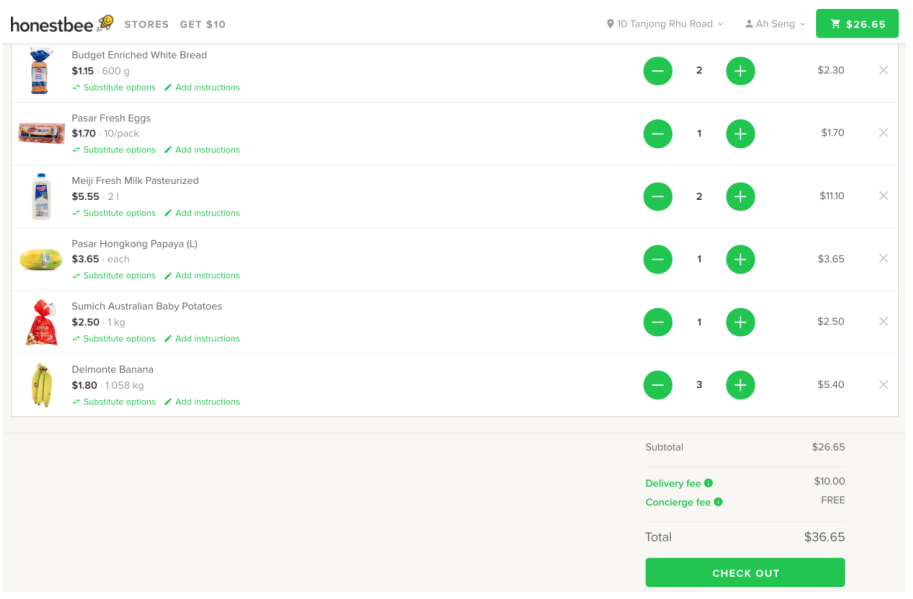
\includegraphics[width=0.6\paperwidth]{C:/Users/Admin/Desktop/Github/question_bank/LyX/static/img/9597-DHS-2016-P2-Q6-1}
\par\end{center}

In the event that the item is out of stock, the customer can also
opt for 3 options: 
\begin{center}
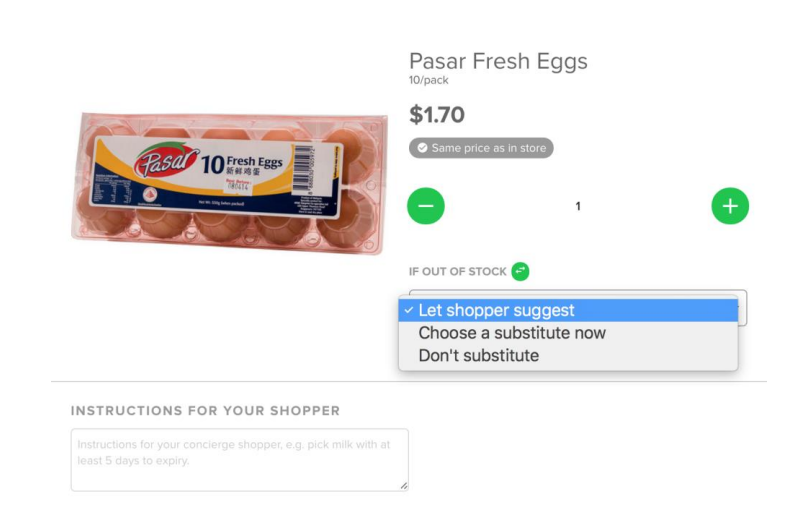
\includegraphics[width=0.6\paperwidth]{C:/Users/Admin/Desktop/Github/question_bank/LyX/static/img/9597-DHS-2016-P2-Q6-2}
\par\end{center}
\begin{enumerate}
\item Produce a normalised relational database schema showing the table
specifications. \hfill{}{[}8{]}
\item Draw an ER diagram illustrating the entities and their relationships.
\hfill{}{[}3{]}
\item Using suitable examples from this context, explain the concepts of
\begin{enumerate}
\item primary key (for the Customer table) \hfill{}{[}2{]}
\item composite key \hfill{}{[}2{]}
\item foreign key \hfill{}{[}2{]}
\end{enumerate}
\item Orders below \$30 is charged a delivery fee of \$10, else delivery
fee is waived. Some orders may incur a concierge fee for special instructions.
Where should fields such as delivery fee and concierge fee be stored?
Why? \hfill{}{[}2{]}
\end{enumerate}
{[}SPLIT\_HERE{]}
\end{enumerate}

\end{document}
